\documentclass[12pt,a4paper]{article}

\usepackage[utf8]{inputenc}
\usepackage{lmodern}
\usepackage[T1]{fontenc}
% paysage
% \usepackage[landscape]{geometry}
\usepackage{lscape}
\usepackage{graphicx}
% \graphicspath{ {images/} }

% headers footers
\usepackage{fancyhdr}
\pagestyle{fancy}

% référencer la dernière page
\usepackage{lastpage}

% pdf
\usepackage{pdfpages}

% francais
% \usepackage[frenchb]{babel}
% math
\usepackage{amssymb}

\usepackage{multicol}
\usepackage{url}

\usepackage{multido}
\usepackage[utf8]{inputenc}
% \usepackage{lmodern}
\usepackage[T1]{fontenc}

\usepackage[sfdefault]{AlegreyaSans} %% Option 'black' gives heavier bold face
%% The 'sfdefault' option to make the base font sans serif
% \renewcommand*\oldstylenums[1]{{\AlegreyaSansOsF #1}}


\usepackage{multicol}
\usepackage[frenchb]{babel}
% \usepackage{pstricks,pst-plot,pst-node}
% \usepackage{pstricks-add}
\usepackage{pst-circ}
\usepackage{pst-magneticfield}
\usepackage{pst-electricfield}
\usepackage{graphicx}
\usepackage{amsmath,amsfonts,amssymb}
\usepackage{titlesec} 
\usepackage{float}
\usepackage{textcomp}
\usepackage{amssymb}
\usepackage[toc,page]{appendix}
\usepackage{listings} 

\lstset{language=Matlab}
\usepackage{lipsum}
\usepackage{enumerate}


%Numerotation par section des équations
\usepackage{amsmath}

\usepackage{tabularx}
\usepackage{longtable}

%------------------------------inclue les références
% \usepackage[nottoc, notlof, notlot]{tocbibind}
%\usepackage{biblatex}
% \usepackage{csquotes}

%\usepackage{etoolbox}
% \patchcmd{\chapter}{\thispagestyle{plain}}{\thispagestyle{fancy}}{}{}
\title{
	\Huge\textsc{Cinematic study of a robot arm}
}
\author{Mohamed Thebti} 

\begin{document}
% retrait de la première ligne d'un paragraphe
\setlength{\parindent}{0mm}

\fancyhead[R]{\slshape \leftmark}
\fancyhead[L]{\slshape Cinematic study of a robot arm}
%\fancyhead[LE,RO]{\slshape \rightmark}
% \fancyhead[LO,RE]{\slshape \leftmark}

% \fancyfoot[C]{Travail de Master}
\fancyfoot[L]{\slshape Thebti Mohamed}
\fancyfoot[C]{}
\fancyfoot[R]{\thepage}

\maketitle
\newpage

\tableofcontents

\newpage



\section{Introduction}


The objective of this report is to study the movement of a robot arm and determine how to compute the position of each articulation. 

This study will give the reader tools needed to engage in the next step, which is a dynamic study. This next step is more complex as it requires notions like inertia, accelerations, ...

\newpage
\section{Robot description}
Different types of robots : anime : human-like machine

A robot is machine composed of parts that is moved using actuator, like electric motor, pneumatic/hydraulic jacks, ...
This actuator is situation in the articulation. 
a computer is integrated in the robot, works as brain, and controls the movement of the arms by sending position and movement orders to each actuator. 
\begin{itemize}
	\item CPU/controller/computer as brain
	\item moving parts
	\item actuators
	\item sensors
\end{itemize}

In this study, we take the simplest robot : 
- robot arm, with several articulation, and 1 actuator in each articulation.

each actuator = liberty degree

the objective : compute 

\newpage
\section{Schéma cinématique}

Robot arm : serial construction : 
This means that the movement of one articulation will influence the position of the next one. 

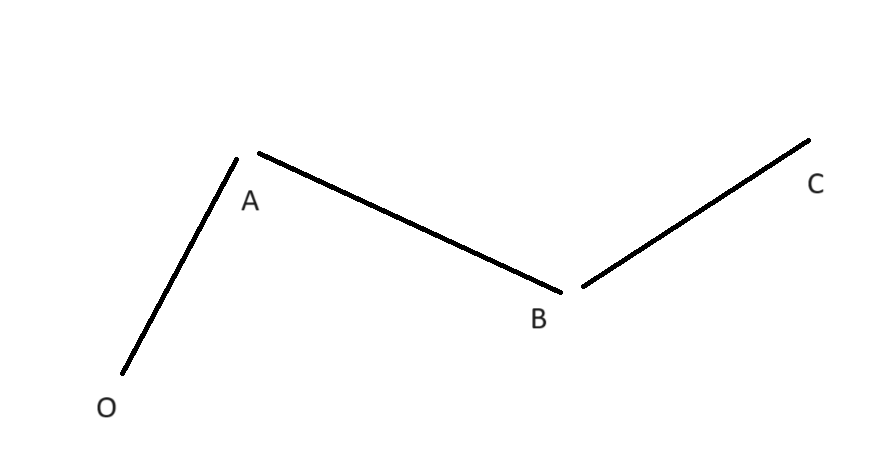
\includegraphics[scale=0.5]{robot_arm.png}

(mettre le schéma du robot ici)
\subsection{Articulations et pivots}
Les articulations : O, A,B,C (head of the robot)
\begin{itemize}
	\item Origin O, A, B : rotation on y axis.
	\item C : Extrémité : rotule et pince
\end{itemize}


ddl : $\alpha_1$, $v_1$ à $v_7$. (v pour vérin)\\


\subsection{Repère global}

Il est placé à l'origine $O$. il se utilisé pour exprimer la position de chaque point, principalement l'extrémité du bras (la pince).
\begin{equation}
R=\{x,y,z\}
\end{equation}
\medbreak
\medbreak

\begin{figure}[H]
	\centering
%	\includegraphics[scale=2]{Vue_dessus.png}
	\caption{Vue de dessus}
\end{figure}

\subsection{Repères locaux}
ce sont des repères mobiles, qui bougent avec les bras sur lesquels ils sont placés. Ainsi chacun dépend du repère précédent : le repère $R_{i+1}$ se déplacent selon un axe du repère $R_i$.
\medbreak

Repère 1 : placé en $A$, rotation de $\alpha_1$ autour de l'axe $z$.
\begin{equation}
R_1=\{x_1,y_1,z_1\}
\end{equation}

\medbreak
Repère 2 : placé en $C$, rotation de $\alpha_2$ autour de l'axe $y_1$.
\begin{equation}
R_2=\{x_2,y_2,z_2\}
\end{equation}


\medbreak
Repère 3 : placé en $D$, rotation de $\alpha_3$ autour de l'axe $y_2$.
\begin{equation}
R_3=\{x_3,y_3,z_3\}
\end{equation}

\medbreak
Repère 4 : placé en $E_1$, rotation de $\alpha_4$ autour de l'axe $y_3$.
\begin{equation}
R_4=\{x_4,y_4,z_4\}
\end{equation}

\medbreak
Repère 5 : placé en $F$, rotation de $\alpha_5$ autour de l'axe $y_4$.
\begin{equation}
R_5=\{x_5,y_5,z_5\}
\end{equation}

\medbreak
Repère 6 : placé en $G$, rotation de $\alpha_6$ autour de l'axe $z_5$.
\begin{equation}
R_5=\{x_5,y_5,z_5\}
\end{equation}

\subsection{Passage d'un repère à un autre}
Matrice de transformation $T_i$ du repère $i+1$ à $i$ : 
\begin{equation}
\vec{A}_{R_i{i+1}}=T_i \cdot \vec{A}_{R_i}
\end{equation}

Pour la suite, nous avons besoin d'exprimer la position d'un point par rapport au repère global. En partant de la relation précédente, on peut en déduire : 
\begin{equation}
\vec{A}_R=T_1 \cdot T_2 \cdot .... \cdot T_i \cdot \vec{A}_{R_i}
\end{equation}

\subsubsection{Matrice de rotation}
Ci-dessous les matrices qui permettent de faire une rotation d'un angle quelconque $\alpha$ selon les axes X, Y et Z. 
\begin{equation}
Rot_X^{\alpha}=
\begin{bmatrix}
1 & 0 & 0\\
0 & cos(\alpha) & -sin(\alpha)\\
0 & sin(\alpha) & cos(\alpha)
\end{bmatrix}
\end{equation}

\begin{equation}
Rot_Y^{\alpha}=
\begin{bmatrix}
cos(\alpha) & 0 & -sin(\alpha)\\
0 & 1 & 0\\
sin(\alpha) & 0 & cos(\alpha)
\end{bmatrix}
\end{equation}

\begin{equation}
Rot_Z^{\alpha}=
\begin{bmatrix}
cos(\alpha) & -sin(\alpha & 0\\
sin(\alpha) & cos(\alpha) & 0\\
0 & 0 & 1
\end{bmatrix}
\end{equation}
\newpage
\section{Etude cinématique}


\subsection{les vecteurs de position}

définir les vecteurs qui expriment les bras du robot, selon les repères définis précédemment. 

\begin{equation}
\vec{OA}_{R_{1}}=
\begin{bmatrix}
0 \\
0\\
l_1
\end{bmatrix}_{R_{1}} \enspace
\vec{AB}_{R_{2}}=
\begin{bmatrix}
0 \\
l_2\\
0
\end{bmatrix}_{R_{2}} \enspace
\vec{BC}_{R_{3}}=
\begin{bmatrix}
l_3 \\
0\\
0
\end{bmatrix}_{R_{3}} \enspace
\vec{CD}_{R_{4}}=
\begin{bmatrix}
0 \\
0\\
-l_4
\end{bmatrix}_{R_{4}} \enspace
\end{equation}

\begin{itemize}
	\item
	\item 
	\item 
\end{itemize}


\medbreak

\medbreak

\medbreak

\medbreak


\subsection{Position des pivots selon repère global}
pour exprimer la position de chaque articulation, multiplie chaque vecteur par les matrices de rotations qui règlent le mvt des articulations depuis la base
\medbreak
explication physique : si le bras 1 bouge, le bras 2 bouge de même. de plus, le bras 2 a son propre mouvement. cece se traduit mathématiquement par une multiplication matricielle.  
\begin{eqnarray}
\vec{OA}_R=\\
\vec{OB}_R=\vec{OA}_R+\vec{AB}_R\\
\vec{OC}_R=\vec{OA}_R+\vec{AB}_R+\vec{B B_1}_R+\vec{B_1 C_1}_R+\vec{C_1 C}_R\\
\vec{OD}_R=\vec{OA}_R+\vec{AB}_R+\vec{B B_1}_R+\vec{B_1 C_1}_R+\vec{C_1 C}_R+\vec{C C_2}_R+\vec{C_2 D}_R
\end{eqnarray}

\begin{equation}
\begin{split}
\vec{OE}_R=\vec{OA}_R+\vec{AB}_R+\vec{B B_1}_R+\vec{B_1 C_1}_R+\vec{C_1 C}_R\\+\vec{C C_2}_R+\vec{C_2 D}_R+\vec{D D_1}_R+\vec{D_1 E}_R
\end{split}
\end{equation}

\begin{equation}
\begin{split}
\vec{OF}_R=\vec{OA}_R+\vec{AB}_R+\vec{B B_1}_R+\vec{B_1 C_1}_R+\vec{C_1 C}_R\\+\vec{C C_2}_R+\vec{C_2 D}_R+\vec{D D_1}_R+\vec{D_1 E}_R+\vec{E F}_R
\end{split}
\end{equation}

\begin{equation}
\begin{split}
\vec{OG}_R=\vec{OA}_R+\vec{AB}_R+\vec{B B_1}_R+\vec{B_1 C_1}_R+\vec{C_1 C}_R+\vec{C C_2}_R\\+\vec{C_2 D}_R+\vec{D D_1}_R+\vec{D_1 E}_R+\vec{E F}_R+\vec{F F_3}_R+\vec{F_3 G}_R
\end{split}
\end{equation}

\begin{equation}
\begin{split}
\vec{OH}_R=\vec{OA}_R+\vec{AB}_R+\vec{B B_1}_R+\vec{B_1 C_1}_R+\vec{C_1 C}_R+\vec{C C_2}_R+\vec{C_2 D}_R\\+\vec{D D_1}_R+\vec{D_1 E}_R+\vec{E F}_R+\vec{F F_3}_R+\vec{F_3 G}_R+\vec{G H}_R
\end{split}
\end{equation}

\subsection{Les quadrilatères du bras}
il y en a six déterminés par : 

\begin{itemize}
	\item $Q_1$ : $B$,$B_1$,$B_2$
	\item $Q_2$ : $C_1$, $C$, $C_2$
	\item $Q_3$ : $D$, $D_4$, $D_5$ et $D$, $D_3$, $D_6$. (symétriques)
	\item $Q_4$ : $D_1$, $D_2$, $E_1$, $E$
	\item $Q_5$ : $E_1$, $E_2$, $F_1$, $F$
	\item $Q_6$ : $F$, $F_1$, $F_2$, $F_3$
	\item $Q_7$ : $G$,$G_1$,$G_2$,$G_3$
\end{itemize}

La relation qui donne les angles et les longueurs de bras pour chaque quadrilatère\footnote{à l'aide des relations de Al-Kashi} : 

\subsubsection{$Q_1$}
\begin{eqnarray}
\frac{v_1}{sin(\beta_5)}=\frac{b_1}{sin(\beta_4)}=\frac{b_2}{sin(\beta_2)}\\
\beta_6=\pi-\beta_1\\
\beta_5=2\pi-\beta_3-\beta_6=2\pi-\beta_3-(\pi-\beta_1)=\pi+\beta_1-\beta_3\\
\pi=\beta_2+\beta_4+\beta_5\\
b_2^2=v_1^2+b_1^2- 2 \cdot v_1 \cdot b_1 \cdot cos(\beta_5)
\end{eqnarray}
Les paramètres constants : $\beta_2$ ,$b_1$,$b_2$
\subsubsection{$Q_2$}
\begin{eqnarray}
\frac{v_2}{sin(\gamma_6)}=\frac{c}{sin(\gamma_8)}=\frac{c_2}{sin(\gamma_4)}\\
\gamma_2=2\pi-\gamma_1\\
\gamma_3=\beta_1\\
\gamma_4=\gamma_1-\beta_1\\
\gamma_6=2\pi-\gamma_5-\beta_6=\pi+\beta_2-\gamma_5\\
\gamma_7=\pi-\gamma_5\\
\gamma_8=2\pi-\gamma_2-\gamma_7\\
\pi=\gamma_4+\gamma_6+\gamma_8\\
c^2=v_2^2+c_2^2- 2 \cdot v_2 \cdot c_2 \cdot cos(\gamma_8)
\end{eqnarray}
\subsubsection{$Q_3$}

\subsubsection{$Q_4$}

\subsubsection{$Q_5$}

\subsubsection{$Q_6$}

\subsubsection{$Q_6$}

Pour résoudre ces quadrilatères et connaître les paramètres inconnus, on utilise la méthode suivante. 
\newpage
\section{La méthode de Newton-Raphson}
but : déterminer les inconnues dans chaque quadrilatère

\begin{itemize}
	\item 
	\item 
	\item 
\end{itemize}


\section{vitesse accélération}


expression générale de la vitesse et de l'accélération

\begin{eqnarray}
v=\frac{d x}{dt}=\frac{d x}{d \omega} \cdot \frac{d \omega}{dt}=\frac{d x}{d \omega} \cdot \dot{\omega}\\
a=\frac{d^2 x}{dt^2}=\frac{dv}{dt}
\end{eqnarray}
Ce qui donne : 


\section{Régulation/contrôle}

\subsection{méthode 1}
connaître le résultat à l'extrémité du bras quand une des variables et modifier : 
\begin{equation}
\delta v \rightarrow \vec{\delta p}
\end{equation}

\subsection{méthode 2}
plus complexe : 
le but est de connaitre les vérins à actionner si on veut que l'extrémité du bras, c'est-à-dire le ..., fasse un certain mouvement

exemple : 
\begin{itemize}
	\item mouvement de translation selon un axe x,y ou z : typiquement imposer que 2 composantes sur les 3 restes constantes
	\item mouvement de rotation : plus complexe
\end{itemize}



\newpage
%\section{Attention aux bâtons dans les roues}

%Étant donné que j'habite en Suisse depuis 1999, j'ai eu pas mal d'expériences dans les activités qui regroupent les jeunes Musulmans, comme le scoutisme au début des années 2000 ou les associations des jeunes à partir de 2005.
%\medbreak
%Toutes ces activités ont été vouées à l'échec car ce sont les anciennes générations de Musulmans, les adultes qui avaient entre 40 et 50 ans, qui contrôlaient ces activités et qui empêchaient les jeunes de devenir indépendants et de prendre la relève pour assurer la suite. 
%\medbreak
%Même les tentatives individuelles initiés par certaines jeunes par la suite, je site comme exemple \textit{Le Bureau des jeunes} vers 2004 et l'association \textit{Jeunes Musulmans de Suisse} en 2006, ont été avortées. Dès qu'une activité qui devient populaire chez les jeunes et qui a du succès inimaginable, elle est visée par ces mêmes adultes car ils ne conçoivent pas qu'une activité puisse être effectuées hors de leurs contrôles. 
\section{Conclusion}


\end{document}